\documentclass[11pt,a4paper]{report}
\usepackage[utf8]{inputenc}
\usepackage[russian]{babel}
\usepackage[OT1]{fontenc}
\usepackage{amsmath}
\usepackage{amsfonts}
\usepackage{amssymb}
\usepackage{graphicx}
\author{Григорий Субботин, Кирилл Муратов, Света Горбунова}
\title{Документация по проекту easySpace}
\begin{document}

\begin{titlepage}
 \begin{center}
    \large
    МИНИСТЕРСТВО ОБРАЗОВАНИЯ И НАУКИ\\ РОССИЙСКОЙ ФЕДЕРАЦИИ
     
    \textit{ФГБОУ ВО Российской Федерации}
    \vspace{0.5cm}
 
    АЛТАЙСКИЙ ГОСУДАРСТВЕННЫЙ УНИВЕРСИТЕТ
    
    \vspace{0.25cm}
     
    \textit{Институт цифровых технологий, электроники и физики}
    
    \vfill 
    Информатика и вычислительная техника
    \vfill
    \textsc{Групповая работа}\\[5mm]
     
    {\LARGE «Разработка графической программы с использованием библиотеки Tkinter, моделирующую солнечную систему»}
  \bigskip
     
     2 курс, группа 595
\end{center}
\vfill
 
\newlength{\ML}
\settowidth{\ML}{«\underline{\hspace{0.6cm}}» \underline{\hspace{1cm}}}
\hfill\begin{minipage}{0.5\textwidth}
  Руководитель курса\\
  \underline{\hspace{\ML}} И.\,А.~Шмаков\\
  «\underline{\hspace{0.5cm}}» \underline{\hspace{1cm}} 2020 г.
\end{minipage}%
\bigskip
 
\hfill\begin{minipage}{0.5\textwidth}
  Студенческая группа:\\
  \underline{\hspace{\ML}} Г.\,М.~Субботин  \\- менеджер проекта\\
  \underline{\hspace{\ML}} К.\,М.~Муратов \\- программист\\
  \underline{\hspace{\ML}} С.\,М.~Горбунова  \\- тестировщик\\
   \underline{\hspace{\ML}} М.\,М.~Воронин  \\- тестировщик\\
\end{minipage}%
\vfill
 
\begin{center}
  Барнаул, 2020 г.
\end{center}
\end{titlepage}

\tableofcontents
\newpage
\section{Теория}
\subsection{Python}

Python – это простой в освоении и мощный язык программирования. Он предоставляет эффективные высокоуровневые структуры данных, а также простой, но эффективный подход к объектно-ориентированному программированию. Его элегантный синтаксис и динамическая типизация наряду с тем, что он является интерпретируемым, делают его идеальным языком для написания сценариев и быстрой разработки приложений в различных областях и на большинстве платформ.

Гвидо ван Россум, создатель языка Python, назвал его так в честь телешоу на BBC под названием «Летающий цирк Монти Пайтона»1, а вовсе не потому, что он любит змей, убивающих животных обвиванием своего длинного тела вокруг них и задавливанием.

Python – простой и минималистичный язык. Чтение хорошей программы на Python очень напоминает чтение английского текста, хотя и достаточно строгого! Такая псевдо-кодовая природа Python является одной из его самых сильных сторон. Она позволяет вам сосредоточиться на решении задачи, а не на самом языке.

Как вы увидите, на Python чрезвычайно легко начать программировать. Python обладает исключительно простым синтаксисом, как уже отмечалось выше.

Python – это пример свободного и открытого программного обеспечения –FLOSS (Free/Libré and Open Source Software). Проще говоря, вы имеете право свободно распространять копии этого программного обеспечения, читать его исходные тексты, вносить изменения, а также использовать его части в своих программах. В основе свободного ПО лежит идея сообщества, которое делится своими знаниями. Это одна из причин, по которым Python так хорош: он был создан и постоянно улучшается сообществом, которое просто хочет сделать его лучше.

При написании программы на Python вам никогда не придётся отвлекаться на такие низкоуровневые детали, как управление памятью, используемой вашей программой, и т.п.

Благодаря своей открытой природе, Python был портирован на много платформ (т.е. изменён таким образом, чтобы работать на них). Все ваши программы смогут запускаться на любой из этих платформ без каких-либо изменений, если только вы избегали использования системно-зависимых функций. Python можно использовать в GNU/Linux, Windows, FreeBSD, Macintosh, Solaris, OS/2, Amiga, AROS, AS/400, BeOS, OS/390, z/OS, Palm OS, QNX, VMS, Psion, Acorn RISC OS, VxWorks, PlayStation, Sharp Zaurus, Windows CE и даже на PocketPC! Вы можете даже использовать такую платформу, как Kivy для создания игр для iOS (iPhone, iPad) и Android.

Программа, написанная на компилируемом языке программирования, как например, C или C++, преобразуется из исходного языка (т.е. C или C++) в язык, понятный компьютеру (бинарный код, т.е. нули и единицы) при помощи компилятора с применением разнообразных флагов и параметров. Когда вы запускаете такую программу, компоновщик/загрузчик копирует программу с диска в оперативную память и запускает её.  Python же, напротив, не требует компиляции в бинарный код. Программа просто выполняется из исходного текста. Python сам преобразует этот исходный текст в некоторую промежуточную форму, называемую байткодом, а затем переводит его на машинный язык и запускает. Всё это заметно облегчает использование Python, поскольку нет необходимости заботиться о компиляции программы, подключении и загрузке нужных библиотек и т. д. Вместе с тем, это делает программы на Python намного более переносимыми, так как достаточно их просто скопировать на другой компьютер, и они работают!

Python поддерживает как процедурно-ориентированное, так и объектно-ориентированное программирование. В процедурно-ориентированных языках программы строятся на основе процедур или функций, которые представляют собой просто-напросто многократно используемые фрагменты программы. В объектно-ориентированных языках программирования программы строятся на основе объектов, объединяющих в себе данные и функционал. Python предоставляет простые, но мощные средства для ООП, особенно в сравнении с такими большими языками программирования, как C++ или Java.

Если вам нужно, чтобы некоторая критическая часть программы работала очень быстро или вы вынуждены скрыть часть алгоритма, вы можете написать эту часть программы на C или C++, а затем вызывать её из программы на Python.

Python можно встраивать в программы на C/C++, чтобы предоставлять возможности написания сценариев их пользователям.

Стандартная библиотека Python просто огромна. Она может помочь в решении самых разнообразных задач, связанных с использованием регулярных выражений, генерированием документации, проверкой блоков кода, распараллеливанием процессов, базами данных, веб-браузерами, CGI, FTP, электронной почтой, XML, XML-RPC, HTML, WAV файлами, криптографией, GUI (графическим интерфейсом пользователя) и другими системно-зависимыми вещами. Помните, что всё это доступно абсолютно везде, где установлен Python. В этом заключается философия Python «Всё включено».

\subsection{Tkinter}
Tkinter – это кроссплатформенная библиотека для разработки графического интерфейса на языке Python (начиная с Python 3.0 переименована в tkinter). Tkinter расшифровывается как Tk interface, и является интерфейсом к Tcl/Tk.

В Python есть довольно много GUI фреймворков (graphical user interface), однако только Tkinter встроен в стандартную библиотеку языка. У Tkinter есть несколько преимуществ. Он кроссплатформенный, поэтому один и тот же код можно использовать на Windows, macOS и Linux.

Визуальные элементы отображаются через собственные элементы текущей операционной системы, поэтому приложения, созданные с помощью Tkinter, выглядят так, как будто они принадлежат той платформе, на которой они работают.

Хотя Tkinter является популярным GUI фреймворком на Python, у него есть свои недостатки. Один из них заключается в том, что графические интерфейсы, созданные с использованием Tkinter, выглядят устаревшими. Если вам нужен современный, броский интерфейс, то Tkinter может оказаться не совсем тем, для этого есть PyQt5 который развивается сильнее в данном плане.

Тем не менее, в плане использования, Tkinter является относительно легким по сравнению с другими библиотеками. Это отличный выбор для создания GUI приложений в Python, особенно если современный облик не в приоритете для программы, а большую роль играет функциональность и кроссплатформенная скорость.

\subsection{Выбранный язык программирования}
Основным языком программирования (далее ЯП) стал Python. Главными факторами при выборе языка стали:
\begin{enumerate}
    \item Высокая скорость написания и прототипирования программы
    \item Относительная легкость чтения кода 
    \item Большое количество документации по языку и дополнительным пакетам
    \item Богатая библиотека пакетов, таких как \textit{Tkinter} 
\end{enumerate} 
\section{Постановка задачи}
Необходимо разработать программу, которая  должна отображать схематичную модель солнечной системы, с указанием информации о каждой  планете, при нажатии на соответствующую планету. 

\section{Цель проекта}
Разработать программу, отображающую модель и поведение солнечной системы. Интерфейс программы должен быть выполнен с использованием библиотеки \textit{Tkinter}. Программа должна быть составлена с использованием парадигмы ООП.

\section{Описание классов}
\subsection{Класс Planet}
Класс Planet  - содержит методы и функции для графического представления планет.
\subsection{Класс UI}
Класс UI - один из классов, в нашей программе. Данный класс предназначен для отрисовки окна с краткой информацией о каждой планете.
Класс UI содержит функции, в которых происходит создание окна  - info, добавление заголовка планеты - Lab, добавление изображения планеты - img. 
Для реализации окна, будем использовать метод \textit{Toplevek},т.е данный способ позволяет создать окно, которое будет всегда находиться поверх основной программы. 
Подобный метод создания окна, в нашем случае, имеет следующие плюсы:
\begin{enumerate}
    \item Возможность открывать несколько окон, к примеру, для сравнения характеристик планет
    \item Модель Солнечной системы, при желании, можно переместить в свободную область, т.о иметь возможность наблюдать модель Солнечной системы и видеть информацию об интерессующей планете
    \item Удобство реализации, т.к в программе будет 2 отдельных окна (основное и окно с информацией)
    \item Более чистый и читаемый код
\end{enumerate}
Рассмотрим подробнее создание окна с информацией:
\begin{verbatim}
===================================================================
#Создаем окно вверхнего уровня
    info = tk.Toplevel(root, bg ='black')
#Задаем заголовок окну. В нашем случае это "Info about planet"
    info.title("Info about planet")
#Устанавливаем размер окна
    info.geometry('800x600')
#Запрещаем пользователю менять размер окна
    info.resizable(False,False)
===================================================================
\end{verbatim}
Вернемся к разработке окна.
Далее установим название планеты, при помощи Label:
\begin{verbatim}
====================================================================
#Выводит имя планеты
    Lab = tk.Label(info,
                    bg = 'black',
                    fg = 'white',
                    text = 'Меркурий', 
                    font = 'Arial 25')
#Упаковываем Label
    Lab.pack()
===================================================================
\end{verbatim}
Теперь в верхней части окна info будет появляться  название планеты.
Помимо названия планеты, необходимо отобразить изображение в окне, т.к информацию лучше "усваивать" наглядно.
Для этого мы использовали метод \textit{PhotoImage}, из библиотеки \textit{Tkinter}:
\begin{verbatim}
#Задаем картинку для планеты
    image1 = tk.PhotoImage(file = 'mercury.gif')
#Присваиваем картинку виджету Label и удаляем границу изображения
    Lab_img = tk.Label(info,image =image1,borderwidth =0)
    Lab_img.image_ref = image1
\end{verbatim}

Поскольку "классический" виджет Label не может нормально отображать многострочный текст, было решено нестандартно использовать виджет Text с некоторыми хитростями. 
С помощью следующего кода можно задать текст, с нужной нам информацией. 
\begin{verbatim}
======================================================================
# Задаем текст  с информацией о планете
    text = tk.Text(info,
            bg = 'black',
            fg = 'white',
            borderwidth = 0 ,
           width = 700, 
            height = 300 , 
            font = 'Arial 10', 
            wrap = 'word', 
           state = 'normal')
#Вставляем текст в  виджет Text    
    text.insert(1.0,'Меркурий — ближайшая к Солнцу планета. 
    Ни воды, ни воздуха на Меркурии нет. 
    \nИз-за того что Меркурий так близок к светилу,
    дневная температура на этой планете почти +450°С.')
#Вставляем текст в  виджет Text        
    text.insert(5.1,'\nФизические характеристики:
    \nРасстояние от солнца - 0,39 астр. ед.;
    \nПериод обращения - 88 дней;
    \nПериод вращения - 58,6 сут.;
    \nДиаметр - 4878 км;
    \nПлотность - 5,5 г/куб.см.')
=====================================================================
\end{verbatim}
 А теперь поговорим о так называемых "костылях". Дело в том, что виджет Text создан для ввода многострочного пользовательского текста, а метод \textit{state = 'normal'}, описаный нами ранее в коде, устанавливает возможность редактирования текста, но если мы установим \textit{state = 'disabled'} текст выводиться не будет. Но если установить сначала значение метода  \textit{state = 'normal'}, а затем ввести следующую строку кода:
 \begin{verbatim}
=====================================================================
     text.configure(state = 'disabled')
=====================================================================
 \end{verbatim}
то мы сможем вывести нужный нам текст, а затем заблокировать пользователю доступ для его редактирования!
С помощью данного "костыля", нами был реализован вывод текста с информацией о каждой планете.
Итоговый код вывода информации о планете, на примере Меркурия, будет выглядеть так:
\begin{verbatim}
====================================================================
class UI:
    def __init__(self):
        pass
     def Mercury(event):#Меркурий
        info = tk.Toplevel(root, width=800,height = 600, bg ='black')        
        info.title("Info about planet") 
        info.geometry('800x600')
        info.resizable(False,False) 
        
        Lab = tk.Label(info, 
                        bg = 'black',
                        fg = 'white',
                        text = 'Меркурий', 
                        font = 'Arial 25')
                        
        image1 = tk.PhotoImage(file = 'mercury.gif')
        Lab_img = tk.Label(info,
                            image =image1,
                            borderwidth =0)
        Lab_img.image_ref = image1
        
        text = tk.Text(info,
                        bg = 'black',
                        fg = 'white', 
                        borderwidth = 0 ,
                        width = 700, 
                        height = 300 , 
                        font = 'Arial 10', 
                        wrap = 'word', 
                        state = 'normal')
        text.insert(1.0,'Меркурий — ближайшая к Солнцу планета. 
        Ни воды, ни воздуха на Меркурии нет. 
        \nИз-за того что Меркурий так близок к светилу, 
        дневная температура на этой планете почти +450°С.')
        text.insert(5.1,'\nФизические характеристики:
        \nРасстояние от солнца - 0,39 астр. ед.;
        \nПериод обращения - 88 дней;
        \nПериод вращения - 58,6 сут.;
        \nДиаметр - 4878 км;
        \nПлотность - 5,5 г/куб.см.')
        
        Lab.pack()
        Lab_img.pack()
        text.pack(side = 'bottom')
        
        text.configure(state = 'disabled')
===================================================================
\end{verbatim}
Остальные планеты реализованы точно таким же образом, меняется только изображение, название планеты и текст.
Итоговый вид окна можно посмотреть в Приложение 1 (рис.1).













\bibliography{Список литературы}


\newpage
\section{Приложение 1}


\begin{figure}[h]
\centering
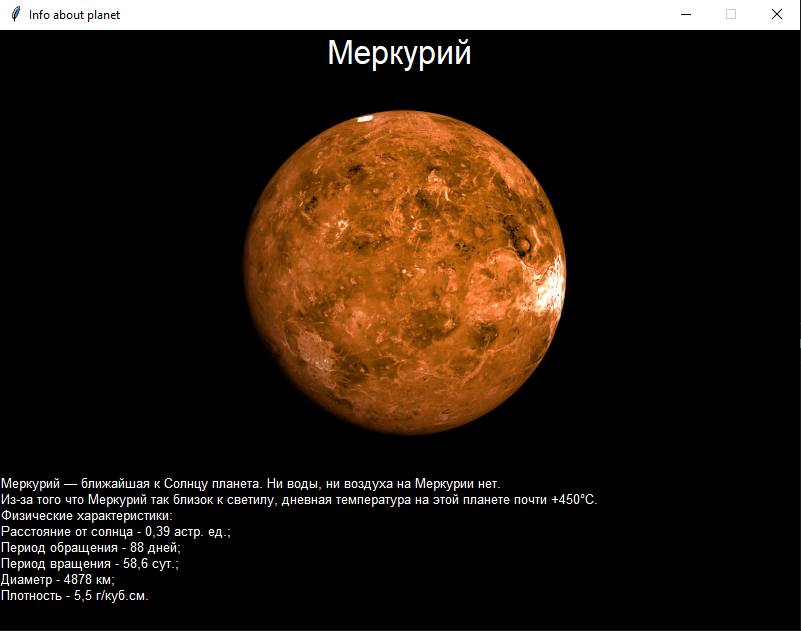
\includegraphics[width=1.0\linewidth]{1.png}
\caption{Итоговый вид окна info about planet}
\label{fig:mpr}
\end{figure}


\section{Приложение 2}


\begin{thebibliography}{5}
\bibitem{Python}
https://www.python.org/
\bibitem{Canvas}
https://younglinux.info/tkinter/menu.php
\bibitem{Wikiversity/Tkinter}
https://ru.wikiversity.org/wiki/Tkinter
\bibitem{Space}
https://v-kosmose.com/planetyi-solnechnoy-sistemyi/
\bibitem{Canvas}
https://webfanat.com/article\_id/?id=117
\end{thebibliography}
\end{document}
